\documentclass[a4paper,12pt]{article}
\usepackage[magyar]{babel}
\usepackage{times}
\usepackage[utf8x]{inputenc}
\usepackage[T1]{fontenc}
\usepackage{lmodern}
\usepackage[intlimits,sumlimits]{amsmath}
\usepackage{amssymb}
\usepackage{graphicx}
\usepackage{hyperref}
% listings begin
\usepackage{color}
\usepackage{xcolor}
\usepackage{listings}
\lstset{literate=%
{Ö}{{\"O}}1
{Ä}{{\"A}}1
{Ü}{{\"U}}1
{ß}{{\ss}}2
{ü}{{\"u}}1
{ä}{{\"a}}1
{ö}{{\"o}}1
{é}{{\'e}}1
{ő}{{\"o}}1
{á}{{\'a}}1
{ó}{{\'o}}1
{í}{{\'i}}1
{ú}{{\'u}}1
{ű}{{\"u}}1
}
\usepackage{caption}
\DeclareCaptionFont{white}{\color{white}}
\DeclareCaptionFormat{listing}{\colorbox{gray}{\parbox{\textwidth}{#1#2#3}}}
\captionsetup[lstlisting]{format=listing,labelfont=white,textfont=white}
% listings end
%opening
\author{MusicSeeker}
\title{Szoftverarchitektúrák NagyHF}
\date{\today}
\begin{document}
%%%%%%%%%%%%%%%%%%%Címoldal%%%%%%%%%%%%%%%%%%%%%%
\begin{titlepage}
\begin{center}
\vspace*{\fill}
\hrulefill\\[0.5cm]
  \textsc{\LARGE Dokumentáció}\\[0.5cm] 
  \textsc{\Large Melyik zeneszolgáltatást válasszam? }\\[0.2cm]
  \textsc{\large Szoftverarchitektúrák tárgy házi feladat}\\[0.5cm]
\hrule
 \end{center}
 \vspace{3cm}
\begin{minipage}{0.6\textwidth}
\begin{flushleft} \large
Készítette:\\[0.2cm]
\textsc{Fekete} Norbert Zoltán\\[0.2cm]
CO0DA1\\
feno26@gmail.com
\end{flushleft}
\end{minipage}
\begin{minipage}{0.6\textwidth}
\begin{flushleft} \large
\vspace{0.82cm}
\textsc{Unicsovics} Milán György\\[0.2cm]
M9GNTV\\
u.milan@gmail.com
\end{flushleft}
\end{minipage}
\vspace*{\fill}
\end{titlepage}
%%%%%%%%%%%%%%%%%%%Szöveg%%%%%%%%%%%%%%%%%%%%%%

\tableofcontents
\newpage

\section{Feladatkiírás}
\label{sec:feladatkiiras}

A felhasználó eszközein (asztali PC vagy mobileszköz) tárolt zenéi alapján a rendszer megadja, hogy melyik zeneszolgáltatás katalógusában (Spotify, Deezer, Google Music,iTunes) található meg a legtöbb a tárolt zenék közül. Ehhez a különböző zeneszolgáltatások API-ját használja fel.

% section feladatkiiras (end)

\section{A fejlesztői csapat}
\label{sec:afejlesztoicsapat}

A csapat tagjai:

\begin{table}[htb]
\begin{center}
\begin{tabular}{|l|l|l|}
\hline
\textbf{Csapattag neve} & \textbf{Neptun-kód} & \textbf{E-mail cím} \\ \hline
Fekete Norbert Zoltán & CO0DA1 & feno26@gmail.com \\ \hline
Unicsovics Milán György & M9GNTV & u.milan@gmail.com \\ \hline
\end{tabular}
\end{center}
\label{tab:acsapattagjai}
\caption{A csapat tagjai}
\end{table}

A csapatban dedikált szerepek kiosztását a csapat kis mérete miatt nem tartottuk fontosnak.

% section afejlesztoicsapat (end)

\section{Részletes feladatleírás}
\label{sec:reszletesfeladatkiiras}

A projekt során célunk egy olyan alkalmazás készítése, amely segít a felhasználónak eligazodni a manapság egyre inkább elterjedő internetes zenei szolgáltatások világában. Ezt a felhasználó meglévő zenei gyűjteményének letapogatásával, majd annak a felhő alapú szolgáltatók készleteivel történő összevetésével éri el.

Az alapvető keresési egység a zenei album lesz. Az elemzési folyamat végeztével a felhasználó egy statisztikát kap, melyből kiolvashatja, mely zeneszolgáltatás gyűjteményével a legnagyobb az átfedés - vagyis mely szolgáltatónál találhat a legkönnyebben a saját stílusának megfelelő zenéket.

Emellett egyszerű, kulcsszavas keresésre is lesz lehetőség (meglévő zenefájlok nélküli kereséshez), amivel kényelmesen lehet majd egyszerre több szolgáltató készletét is lekérdezni.

A program első megközelítésben a \textit{Deezer}, a \textit{Spotify}, az \textit{iTunes} és a \textit{Last.Fm} szolgáltatásait fogja támogatni, de célunk egy általános architektúra kialakítása, mely később könnyedén bővíthető további szolgáltatásokkal (pl.: \textit{Google Play Music}).

% section reszletesfeladatkiiras (end)

\section{Technikai paraméterek}
\label{sec:technikaiparameterek}

A definiált alkalmazást Python platformra készítjük el annak érdekében, hogy több operációs rendszeren (Windows, Linux, Mac OS) is lehessen használni.  Szükség lesz ezen kívül néhány Python-os könyvtárhoz, ezeket a Python csomagkezelőjével (\textit{pip}) egyszerűen lehet majd telepíteni.

A program felhasználói felületét \href{http://python-gtk-3-tutorial.readthedocs.org/en/latest/}{Python GTK+ 3} segítségével fogjuk elkészíteni, a GUI-t magát deklaratív módon \href{https://glade.gnome.org/}{Glade} segítségével állítjuk elő.

Külső függőségeink közé tartoznak a zeneszolgáltatások API-jai is:

\begin{itemize}
	\item \href{https://developer.spotify.com/web-api/}{Spotify}
    \item \href{http://developers.deezer.com/api/}{Deezer}
    \item \href{https://www.apple.com/itunes/affiliates/resources/documentation/itunes-store-web-service-search-api.html}{iTunes}
    \item \href{http://www.last.fm/api}{Last.fm}
    \item \href{http://unofficial-google-music-api.readthedocs.org/en/latest/}{(Google Music)}
\end{itemize}

A fent felsorolt külső függőségek sebességének függvényében, lehet, hogy szükség lesz valamilyen szerver oldali komponens fejlesztésére is, amely egy fajta cache-ként szolgálva gyorsíthatja a program működését. A szerver elérhetősége viszont a program funkcionalitását nem befolyásolja.

% section technikaiparameterek (end)

\section{Szótár}
\label{sec:szotar}

% section szotar (end)

\begin{description}
    \item[Zeneszolgáltatás] Kereskedelmi streamelő alkalmazás, melyben a fehasználó zenéket hallgathat illetve vásárolhat.
    \item[Zeneállomány] A zeneszolgáltatás vagy a felhasználó által birtokolt zenealbumok összessége.
    \item[Zenei katalógus] A zeneszolgáltatás kereshető zeneállománya.
    \item[Kiértékelési statisztika] A felhasználó által megtekinthető grafikus szemléltető eszköz, mely arra szolgál, hogy az egyes zeneszolgáltatásoknál, mely zenealbumok érhetőek el.
    \item[Zeneállomány felderítése] A felhasználó által megadott helyen az elérhető zenealbumok és azok adatainak összegyűjtése.
    \item[Keresés zenékre] Minden támogatott zeneszolgáltató átvizsgálása, hogy egy bizonyos zenealbum elérhető-e az adott platformon.
\end{description}

\section{Essential use-case-ek}
\label{sec:usecaseek}

\subsection{Use-case diagram}
\label{sub:ucdiagram}

\begin{figure}[htp]
\centering
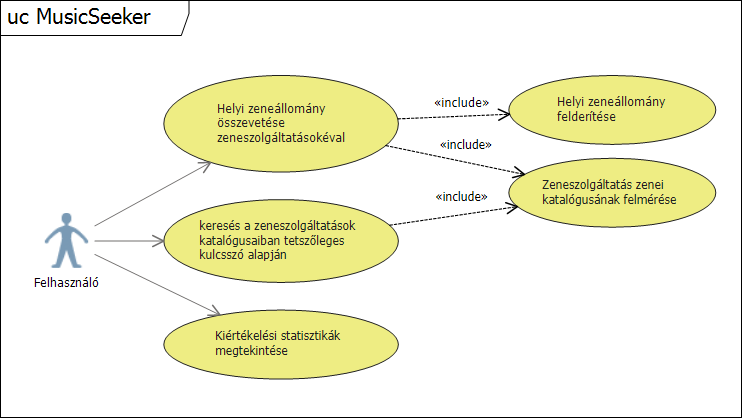
\includegraphics[scale=0.8]{img/01_UseCases.png}
\caption{A MusicSeeker use case diagramja}
\label{fig:01_UseCases}
\end{figure}


% subsection ucdiagram (end)

% section usecaseek (end)

\section{Rendszerterv}
\label{sec:documentation}

\subsection{A rendszer célja, funkciói és környezete}
\label{sub:arendszercelja}

\subsubsection{Feladatkiírás}
\label{ssub:feladatkiiras}

A felhasználó eszközein (asztali PC vagy mobileszköz) tárolt zenéi alapján a rendszer megadja, hogy melyik zeneszolgáltatás katalógusában (Spotify, Deezer, Google Music, iTunes) található meg a legtöbb a tárolt zenék közül. Ehhez a különböző zeneszolgáltatások API-ját használja fel. 
A feladat részletes specifikációja a követelményspecifikáció dokumentumban olvasható.

% subsubsection feladatkiiras (end)

\subsubsection{A rendszer által biztosítandó tipikus funkciók }
\label{ssub:arendszeraltalbiztositandofunkciok}

Vázlatosan az alábbi funkciók biztosítását várjuk el a rendszertől. (A funkciók részletes definíciója szintén a követelményspecifikáció dokumentumban olvasható.) 

\begin{itemize}
	\item helyi zeneállomány összevetése zeneszolgáltatásokéval, melynek lépései:
		\begin{itemize}
			\item helyi zeneállomány felderítése 
			\item zeneszolgáltatások katalógusainak felmérése 
			\item kiértékelési statisztika megjelenítése, szolgáltatóajánlás
		\end{itemize}
	\item keresés a zeneszolgáltatások katalógusaiban tetszőleges kulcsszó alapján
\end{itemize}

% subsubsection arendszeraltalbiztositandofunkciok (end)

\subsubsection{A program környezete}
\label{ssub:aprogramkornyezete}

A szoftvert vastagkliens alkalmazásként készítettük el. Annak érdekében, hogy több operációs rendszeren (Windows, Linux, Mac OS X stb.) is futtatható legyen, platformfüggetlen megoldásokat választottunk. Az alkalmazást Python platformra készítettük el. Szükséges ezen kívül néhány Python könyvtár telepítése is, ami a Python csomagkezelőjével (\texttt{pip}) egyszerűen megtehető. A felhasznált csomagok a következőek:

\begin{itemize}
	\item \href{https://code.google.com/p/stagger/}{Stagger}
	\item \href{http://docs.python-requests.org/}{Requests}
\end{itemize}

A program felhasználói felületét Python GTK+ 3 segítségével készítettük el, így a GTK grafikus könyvtár telepítése is szükséges.

Külső függőségeink közé tartoznak a zeneszolgáltatások is: 
\begin{itemize}
	\item \href{https://developer.spotify.com/web-api/}{Spotify}
    \item \href{http://developers.deezer.com/api/}{Deezer}
    \item \href{https://www.apple.com/itunes/affiliates/resources/documentation/itunes-store-web-service-search-api.html}{iTunes}
    \item \href{http://www.last.fm/api}{Last.fm}
\end{itemize}
Ezen szolgáltatások eléréséhez természetesen internetkapcsolat szükséges.

% subsubsection aprogramkornyezete (end)

% subsection arendszercelja (end)

\subsection{Tervezés és implementáció}
\label{sub:tervezesesimplementacio}

Az alkalmazást a skálázhatóság és továbbfejleszthetőség miatt egy többrétegű alkalmazásként készítettük el. Az egyes rétegek jól definiáltan különválnak egymástól.
 
Az általunk elkészített programot MusicSeeker-nek neveztük el, mely névvel az alkalmazás legfőbb funkciójára akartunk utalni, a zenék keresésére.

A fejezetben áttekintést adunk a program architektúrájáról, bemutatjuk az egyes komponensek feladatait és felelősségeit, illetve ismertetjük a grafikus felhasználói felület felépítését.

\subsubsection{Architektúra}
\label{ssub:architektura}

A MusicSeeker architektúrája 4 rétegre bontható fel:

\begin{itemize}
	\item adatréteg
	\item adatelérési réteg
	\item üzleti logikai réteg
	\item felhasználói felület
\end{itemize}

\begin{figure}[htp]
\centering
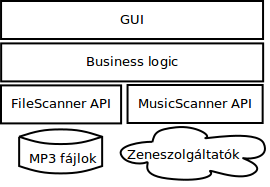
\includegraphics[scale=0.6]{img/architecture.png}
\caption{A MusicSeeker architektúrája}
\label{fig:architecture}
\end{figure}

Az egyes rétegek célját és tervezési szempontjait a következő alfejezetekben fogjuk ismertetni. A különböző rétegek tervezésekor használt mintákat, pedig az alkalmazás alábbi, magasszintű osztálydiagrammján szemléltetjük.

\begin{figure}[htp]
\centering
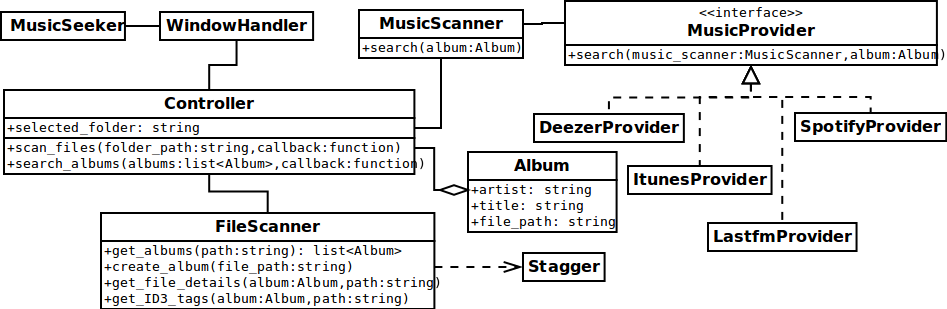
\includegraphics[scale=0.4]{img/class.png}
\caption{A MusicSeeker magasszintű osztálydiagrammja}
\label{fig:class}
\end{figure}

\paragraph{Adatréteg}
\label{par:adatreteg}

\subparagraph{Célja:}

Adatok szolgáltatása a felsőbb rétegek számára, zenékről és zeneszolgáltatások könyvtárairól.

A hagyományos adatbázis réteget itt egy főleg külső komponensekből álló réteg alkotja, hiszen a program működéséhez szükséges adatok, minden esetben felhasználói beavatkozásra, on-the-fly lesznek összegyűjtve.

A gépen található zenealbumok adatai, a lokális gépről tallózott mappából, az MP3 fájlokat kigyűjtve és elemezve lesznek meghatározva.

A felhőben található zeneszolgáltatások könyvtárának adatai, azok API-jainak felhasználásával lesznek összegyűjtve.

% paragraph adatreteg (end)

\paragraph{Adathozzáférési réteg (Data Access Layer)}
\label{par:dal}

\subparagraph{Célja:}

Az adathozzáférési réteg két részből áll, egyrészt a lokális gépen található zenék metaadataihoz és a felhőben található zeneszolgáltatások könyvtárainak adataihoz nyújtanak hozzáférést.

\begin{description}
	\item[FileScanner API] Ezen a komponensen keresztül lehet a lokális gépről elérhető zenék metaadatait lekérdezni, azok ID3 címkéinek kiolvasásával, majd a megszerzett adatokból az alkalmazás központi szerepét játszó entitás példányait létrehozni.

\textbf{Megvalósítás:}
A FileScanner \texttt{get\_albums} függvényét meghívva megkeresi egy adott mappában az összes MP3 fájlt, majd azok ID3 címkét kiolvassa és Album példányokból álló listát ad vissza. Működését tekintve a FacadeWrapper mintát valósítja meg, ugyanis egy külső Stagger nevű könyvtár kezelését fedi el az ID3 címkék kiolvasásakor. Az Album példányok elkészítését Builder mintával készítettük el, hogy a továbbfejlesztéskor ezek az entitások könnyen kiegészíthetőek legyenek új attribútumokkal, amelyeket változatos módokon lehet beszerezni.
	\item[MusicScanner API] A MusicScanner arra szolgál, hogy a felhőben található zeneszolgáltatók könyvtáraiból adatokat tudjunk szerezni. Ezt elsősorban arra fogjuk használni, hogy megvizsgáljuk, hogy a lokális gépen elérhető zenealbumok megtalálhatóak-e az adott zeneszolgáltatásban.

\textbf{Megvalósítás:}
A MusicScanner működése a Visitor minta alapján lett megvalósítva. A minta terminológiáját tekintve a különböző zeneszolgáltatók adatszolgáltató osztályai lesznek a visitorok, amelyek adatokat tudnak szerezni különböző albumokról. Így a rendszer tetszőlegesen kibővíthető új zeneszolgáltatásokkal, de a MusicProvideren keresztül új funkciók is fejleszthetők a rendszerbe.

A különböző zeneszolgáltatások közül végül 4-et választottunk ki, és építettünk be az alkalmazásba:
\begin{itemize}
	\item Deezer
	\item iTunes
	\item Last.fm
	\item Spotify
\end{itemize}

Ezekre azért esett a választás, mert nagyon egyszerű REST API-hoz hasonló, webes elérési felületük van, melyet nagyon egyszerűen tudtunk implementálni. A webszolgáltatások meghívásához a requests könyvtárat használtuk fel. A Last.fm kivételével minden szolgáltatás regisztráció nélkül is használható, a használatához kötődő kvótákat megvizsgálva úgy döntöttünk, hogy nem szükséges a követelményspecifikációban említett cache szolgáltatás implementálása.
\end{description}

% paragraph dal (end)

\paragraph{Üzleti logikai réteg (Business Logic Layer)}
\label{par:bll}

\subparagraph{Célja:} Az üzleti logikai réteg felel a különböző fő használati esetek végrehajtásáért, ezek pedig a helyi állomány vizsgálata, és információk gyűjtése felhőszolgáltatóktól, és statisztika készítése az eredmények alapján. Ezen tevékenységeket az alatta levő rétegeket használva éri el.

\textbf{Megvalósítás:}
A zenei albumokkal kapcsolatos adatok gyűjtését a Controller osztály valósítja meg, mind a helyi zeneállomány, mind a zeneszolgáltatásokban található információk alapján. Statisztikák készítéséért a Statistics osztály felelős.

% paragraph bll (end)

\paragraph{Grafikus felhasználói felület}
\label{par:gui}

\subparagraph{Célja:}
A grafikus felület felelős a felhasználóval való interakcióért. A felhasználó végrehajthat műveleteket, és azok eredményéről tájékoztatást kap.

\textbf{Megvalósítás:}
Maga a grafikus felület gyakorlatilag teljes egészében deklaratív módon Glade segítségével lett megvalósítva. A felülethez kapcsolódó eseménykezelőket a WindowHandler osztály valósítja meg, valamint az üzleti logikai réteg által létrehozott eredményeket jeleníti meg a felhasználó számára.
A hosszan futó feladatokat a Future minta segítségével háttérszálon végeztük el, és a felhasználót folyamatosan tájékoztattuk a végrehajtani kívánt folyamat állapotáról.

% paragraph gui (end)

% subsubsection architektura (end)

\subsubsection{Adatterv}
\label{ssub:adatterv}

\paragraph{Album entitás}
\label{par:album}

\begin{figure}[htp]
\centering
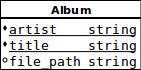
\includegraphics[scale=0.6]{img/album.png}
\caption{Album entitás}
\label{fig:album}
\end{figure}

Az alkalmazás működésében központi szerepet tölt be, és gyakorlatilag egyetlen entitásként létezik az Album, mely egy zenei albumot jelöl. A zenei albumot, annak előadója és címe azonosítja, egyéb attribútuma még az útvonal is, melyen keresztül elérhető a fájlrendszerben.

% paragraph album (end)

% subsubsection adatterv (end)

\subsubsection{GUI-terv}
\label{ssub:guidesign}

Amikor a felhasználó elindítja az alkalmazást, egy üdvözlőképernyő fogadja (\ref{fig:scrstart}.~ábra). A specifikációban kijelölt két fő usecase-nek megfelelően két fő menüpont fogadja: egy, amellyel egyszerű, kulcsszó alapú kereséseket végezhet a támogatott felhőszolgáltatók adatbázisán, és egy másik, amellyel komplex letapogatást és összehasonlítást végezhet, a saját, meglévő zenei gyűjteménye alapján.

\begin{figure}[htp]
\centering
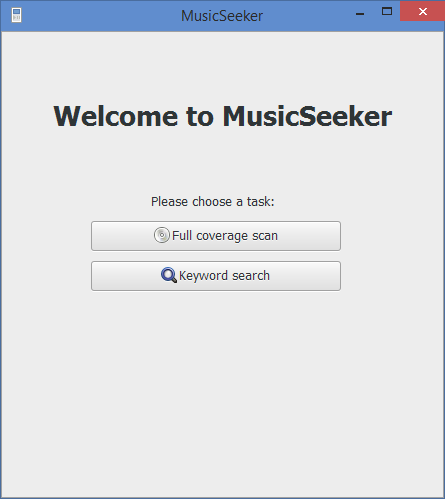
\includegraphics[scale=0.4]{img/screenshots/screenshot01.png}
\caption{A MusicSeeker kezdőképernyő}
\label{fig:scrstart}
\end{figure}

A felhasználó a két gomb segítségével juthat a konkrét funkciókhoz tartozó képernyőkre, ahonnan az ottani Home gomb segítségével bármikor visszatalálhat.

A Full coverage scan egy összetettebb funkció, ezért egy varázsló jellegű felületet kapott (\ref{fig:scrscan}.~ábra).

A legelső lépés, hogy a felhasználó szkennelje a lokális zenei gyűjteményét. Ehhez  csupán a megfelelő mappát kell kiválasztania, majd a Scan gombra kattintania. Ekkor az alkalmazás rekurzívan összegyűjti a mappa alatt található valamennyi mp3 fájl albuminformációját, amit a művelet végeztével egy egyszerű táblázatban meg is jelenít.

\begin{figure}[htp]
\centering
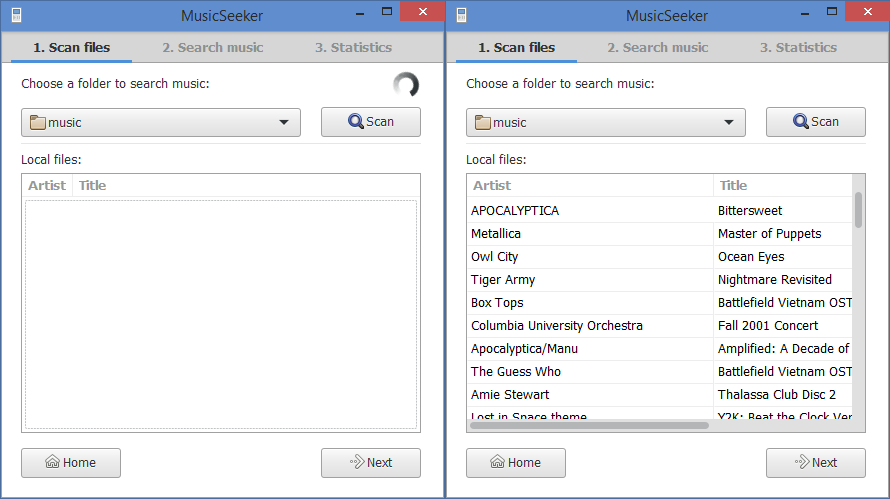
\includegraphics[scale=0.4]{img/screenshots/screenshot02.png}
\caption{Lokális gyűjtemény letapogatása}
\label{fig:scrscan}
\end{figure}

A táblázat megtekintése után a Next gomb továbbvezeti a felhasználót a következő lépéshez, amely már a felhőszolgáltatók tényleges lekérdezése (\ref{fig:scrsearch}.~ábra).

\begin{figure}[htp]
\centering
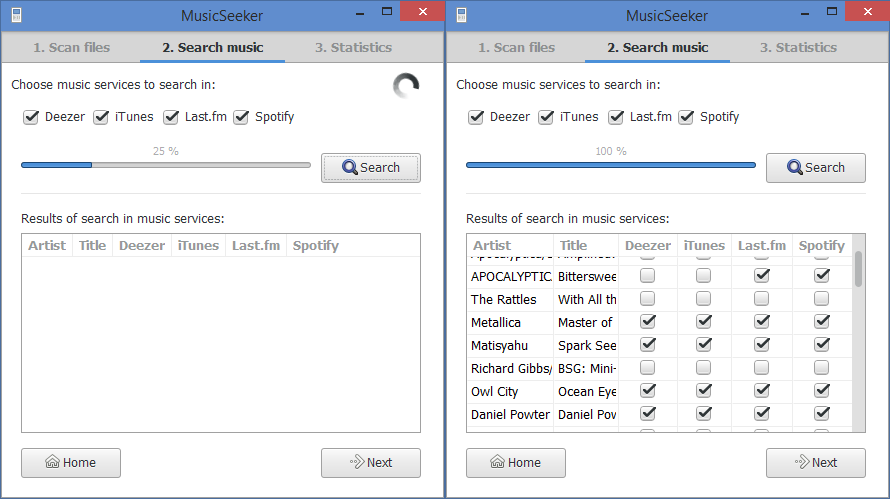
\includegraphics[scale=0.4]{img/screenshots/screenshot03.png}
\caption{Zeneszolgáltatók letapogatása}
\label{fig:scrsearch}
\end{figure}

Ez a lépés már több időt vesz igénybe, mivel a szolgáltatók általában korlátozzák a másodpercenként küldhető kérések számát. Ezért ezen a felületen elhelyeztünk egy progressbart, mely a lekérdezések állapotát jelzi.

A keresés előtt a felhasználó egyszerű checkboxokkal választhatja ki, a támogatott szolgáltatók közül melyek kínálata érdekli.

A letapogatás befejeztével táblázatos formában jelenítjük meg az eredményeket: az egyes lokálisan felderített albumok mellett egy-egy checkboxszal jelöljük, mely szolgáltatóknál érhetők el.

A Next gomb itt már a végső nézethez, a statisztikákhoz vezet (\ref{fig:scrstat}.~ábra). Ezen az oldalon a keresés aggregált eredménye látszik, vagyis hogy melyik szolgáltatónál mennyi található meg az albumainkból.
Az adatok alapján tippet adunk a felhasználónak, melyik zeneszolgáltatót érdemes választania, ha szeretne előfizetni - azaz melyik szolgáltatóval legnagyobb az átfedés.

\begin{figure}[htp]
\centering
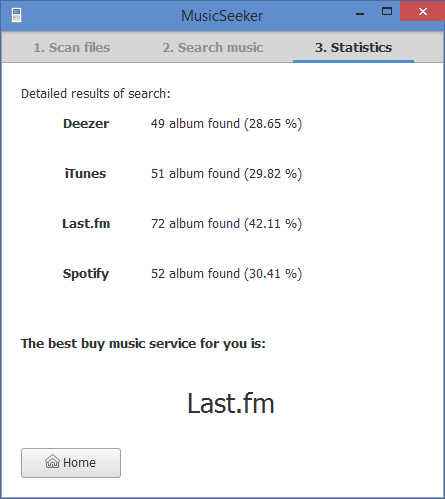
\includegraphics[scale=0.4]{img/screenshots/screenshot04.png}
\caption{Statisztika nézet a letapogatás után}
\label{fig:scrstat}
\end{figure}

Az alkalmazás másik fő funkciója, a kulcsszavas keresés jóval egyszerűbb, mindössze egy oldalas (\ref{fig:scrkword}.~ábra). A szolgáltatókat itt is checkboxokkal választhatjuk ki. A kívánt szerző illetve album nevét beírva, majd a Search gombra kattintva lefut a lekérdezés. A szolgáltatók nevei mellett zöld illetve piros kör jelzi, hogy a kulcsszavarka érkezett-e találat az adott szolgáltató rendszeréből.

\begin{figure}[htp]
\centering
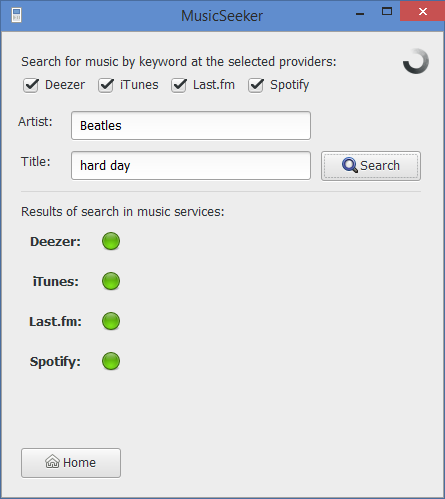
\includegraphics[scale=0.4]{img/screenshots/screenshot05.png}
\caption{Kulcsszavas keresés a zeneszolgáltatóknál}
\label{fig:scrkword}
\end{figure}

% subsubsection guidesign (end)

% subsection tervezesesimplementacio (end)

\subsection{Telepítési leírás}
\label{sub:telepitesileiras}

A Python program interpretált futtatásához a Python futtatókörnyezet 3.x verziója szükséges. A Python könyvtárak telepítéséhez a \texttt{pip} nevű csomagkezelő program telepítése ajánlott.

A szükséges könyvtárak a programhoz csatolt \texttt{requirements.txt} nevű fájlban találhatóak meg, amelyeket a \texttt{pip} nevű program fel tud dolgozni, és telepíti a megfelelő könyvtárakat.

\subsubsection{Linux}
\label{ssub:linux}

\begin{lstlisting}[label={lst:install}, caption=Telepítés Linux környezetben,breaklines=true]
sudo apt-get install python3-all python3-all-dev python3-gi python-glade2
sudo pip -r requirements.txt
\end{lstlisting}

% subsection linux (end)

\subsubsection{Windows}
\label{ssub:windows}

CPython környezet megfelelőverziójának telepítése: \url{http://python.org/download}

Ha véletlen probléma adódik a Stagger nevű könyvtárral, azt manuálisan kell telepíteni az alábbi címről: \url{https://pypi.python.org/pypi/stagger/0.4.2}

A grafikus felület működéséhez a Python mellett szükséges a GTK grafikus könyvtár is. Windows esetén mi a következő telepítőkészletet használtuk:
\url{http://sourceforge.net/projects/pygobjectwin32/}
Ez nem csak magát a GTK-t tartalmazza, hanem különböző  - többek között Pythonhoz szükséges - fejlesztőeszközöket is, ezek telepítése a főprogram futtatásához opcionális.

% subsubsection windows (end)

% subsection telepitesileiras (end)

\subsection{A program készítése során felhasznált eszközök}
\label{sub:aprogramkeszitesesoranfelhasznalt}

\begin{description}
	\item[\href{https://glade.gnome.org/}{Glade}] Segítség GTK-s felületek egyszerűbb, XML alapú előállításához. Grafikus designert is tartalmaz. Windows-on a fent említett összevont telepítőkészletnek (PyGObjectWin32) is része.
	\item[\href{https://github.com/}{GitHub}] Verziókezelés.
	\item[\href{http://www.skype.com/hu/}{Skype}] Kommunikáció, kapcsolattartás.
\end{description}

\subsubsection{Linux}
\label{ssub:linux}

\begin{description}
	\item[\href{http://www.sublimetext.com/3}{Sublime Text3}] Könnyűsúlyú kiterjeszthető szövegkezelő, mely IDE-ként is megállja a helyét.
	\item[\href{http://editorconfig.org/}{EditorConfig}] Egységes IDE beállítások kezelésére alkalmas konfigurációs formátum.
\end{description}

% subsubsection linux (end)

\subsubsection{Windows}
\label{ssub:windows}

\begin{description}
	\item[\href{http://pytools.codeplex.com/wikipage?title=PTVS\%20Installation}{Python Tools for Visual Studio}] Integrált fejlesztőkörnyezet Pythonhoz
\end{description}

% subsubsection windows (end)

% subsection aprogramkeszitesesoranfelhasznalt (end)

\subsection{Továbbfejlesztési lehetőségek}
\label{sub:tovabbfejlesztes}

A program feladatának egyszerűségéből adódóan leginkább felületi fejlesztéseket lehetne még elvégezni:

\begin{itemize}
	\item Felületi elemek dinamikus átmérezetése.
	\item Ergonómikusabb táblázatok, illetve checkbox-ok, nagyobb mennyiségű támogatott zeneszolgáltatás esetén.
	\item Statisztikai nézet továbbfejlesztése, esetleg más jellegű aggregált adatok kijelzése.
	\item Minél több zeneszolgáltatás integrációja.
\end{itemize}

% subsection tovabbfejlesztes (end)

\subsection{Összefoglalás}
\label{sub:osszefoglalas}

Munkánk során megterveztük, implementáltuk és dokumentáltuk a Music-Seeker nevű alkalmazást, mely segít a felhasználónak saját ízlésének megfelelő zeneszolgáltatót választani, meglévő zenei gyűjteménye alapján.

Az alkalmazás 3 rétegű architektúrát használ: adatelérési réteg, logikai réteg és grafikus felhasználói felület. A helyi adatokat a felhasználó meglévő mp3 fájljaiból olvassa ki, a stagger könyvtár segítségével. A zeneszolgáltatók katalógusait azok REST interfészén keresztül éri el. A grafikus felület a GTK könyvtárat használja.

Bízunk benne, hogy munkánk eredményeként egy hasznos kis programot kaptunk, mely segítséget nyújthat a zeneszolgáltatást kereső embereknek, hogy azok a számukra lehető legmegfelelőbb tartalomhoz juthassanak hozzá a pénzükért.

% subsection osszefoglalas (end)

\subsection{Hivatkozások}
\label{sub:hivatkozasok}

\begin{itemize}
	\item CPython: \url{http://python.org/}
	\item PyGObjectWin32: \url{http://sourceforge.net/projects/pygobjectwin32/}
	\item Glade: \url{https://glade.gnome.org/}
	\item Stagger: \url{https://pypi.python.org/pypi/stagger/0.4.2}
	\item Requests: \url{http://docs.python-requests.org/}
	\item Sublime Text3: \url{http://www.sublimetext.com/3}
	\item EditorConfig: \url{http://editorconfig.org/}
	\item PTVS: \url{http://pytools.codeplex.com/}
	\item GitHub: \url{https://github.com/}
	\item Skype: \url{http://www.skype.com/}
\end{itemize}

% subsection hivatkozasok (end)
  
% section documentation (end)

\end{document}
